\documentclass{standalone}
\usepackage{tikz}
\usetikzlibrary{patterns, positioning}


\begin{document}
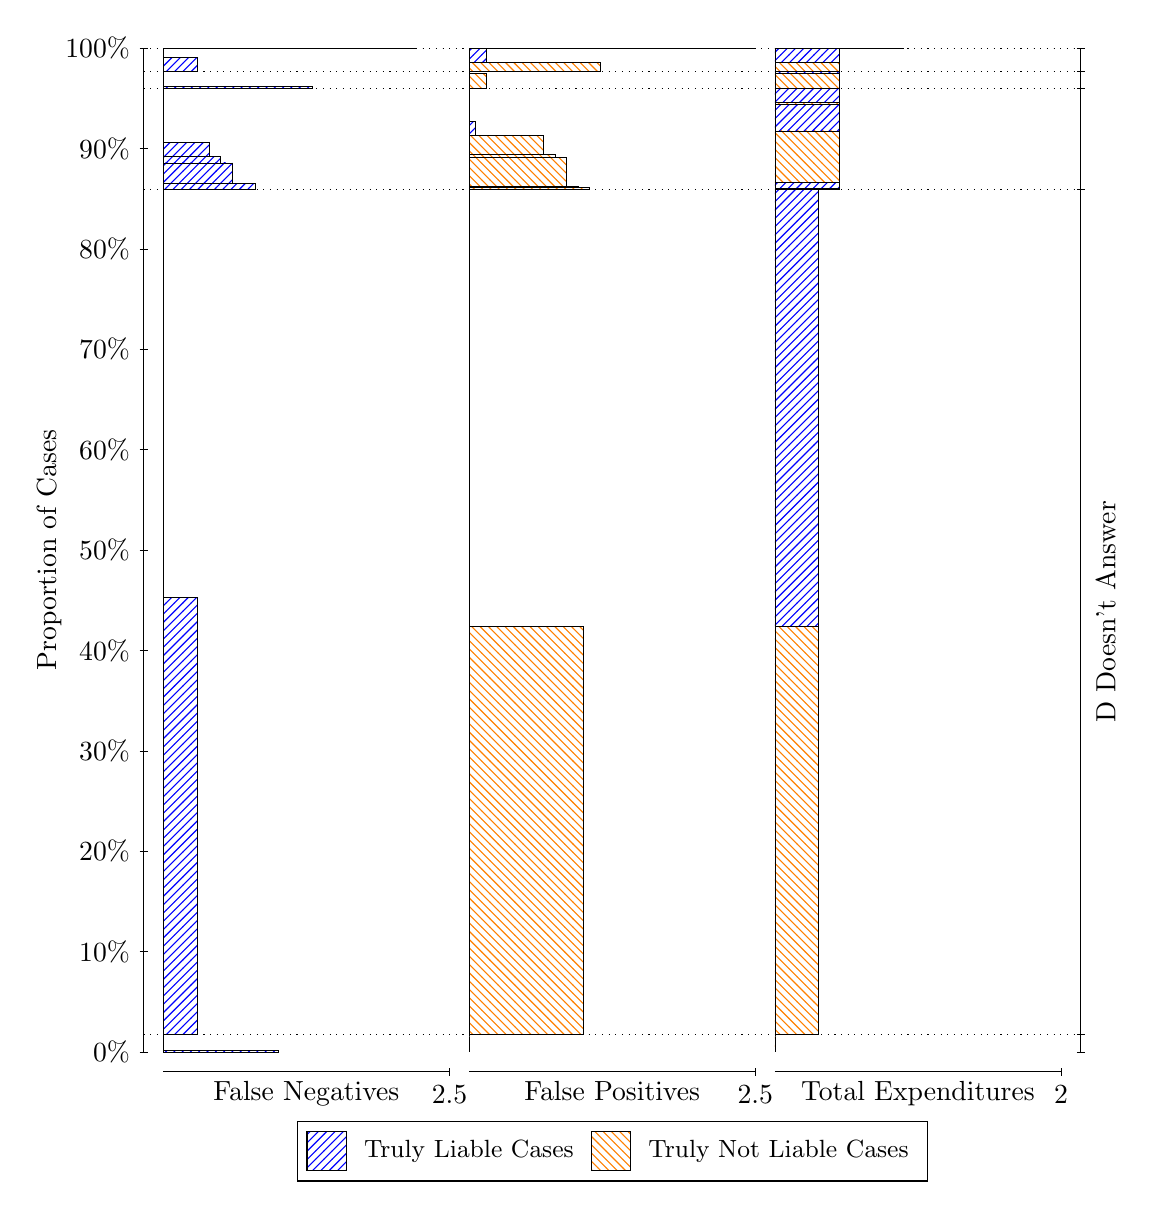
\begin{tikzpicture}
\draw[black, very thin] (1.5,1.75) -- (1.5,14.5);
\node[rotate=90, text=black, anchor=center] at (0.3, 8.125) {Proportion of Cases};
\draw[black, very thin] (1.45,1.75) -- (1.55,1.75);
\node[text=black, anchor=east] at (1.45, 1.75) {0\%};
\draw[black, very thin] (1.45,3.025) -- (1.55,3.025);
\node[text=black, anchor=east] at (1.45, 3.025) {10\%};
\draw[black, very thin] (1.45,4.3) -- (1.55,4.3);
\node[text=black, anchor=east] at (1.45, 4.3) {20\%};
\draw[black, very thin] (1.45,5.575) -- (1.55,5.575);
\node[text=black, anchor=east] at (1.45, 5.575) {30\%};
\draw[black, very thin] (1.45,6.85) -- (1.55,6.85);
\node[text=black, anchor=east] at (1.45, 6.85) {40\%};
\draw[black, very thin] (1.45,8.125) -- (1.55,8.125);
\node[text=black, anchor=east] at (1.45, 8.125) {50\%};
\draw[black, very thin] (1.45,9.4) -- (1.55,9.4);
\node[text=black, anchor=east] at (1.45, 9.4) {60\%};
\draw[black, very thin] (1.45,10.675) -- (1.55,10.675);
\node[text=black, anchor=east] at (1.45, 10.675) {70\%};
\draw[black, very thin] (1.45,11.95) -- (1.55,11.95);
\node[text=black, anchor=east] at (1.45, 11.95) {80\%};
\draw[black, very thin] (1.45,13.225) -- (1.55,13.225);
\node[text=black, anchor=east] at (1.45, 13.225) {90\%};
\draw[black, very thin] (1.45,14.5) -- (1.55,14.5);
\node[text=black, anchor=east] at (1.45, 14.5) {100\%};

\draw[black, very thin] (13.4,1.75) -- (13.4,14.5);
\draw[black, very thin] (13.35,1.75) -- (13.45,1.75);
\node[anchor=west] at (13.35, 1.75) {};
\draw[black, very thin] (13.35,1.9699) -- (13.45,1.9699);
\node[anchor=west] at (13.35, 1.9699) {};
\draw[black, very thin] (13.35,12.705) -- (13.45,12.705);
\node[anchor=west] at (13.35, 12.705) {};
\draw[black, very thin] (13.35,13.984) -- (13.45,13.984);
\node[anchor=west] at (13.35, 13.984) {};
\draw[black, very thin] (13.35,14.206) -- (13.45,14.206);
\node[anchor=west] at (13.35, 14.206) {};
\draw[black, very thin] (13.35,14.491) -- (13.45,14.491);
\node[anchor=west] at (13.35, 14.491) {};
\draw[black, very thin] (13.35,14.497) -- (13.45,14.497);
\node[anchor=west] at (13.35, 14.497) {};
\draw[black, very thin] (13.35,14.5) -- (13.45,14.5);
\node[anchor=west] at (13.35, 14.5) {};

\draw[black, very thin, pattern color=blue, pattern=north east lines] (1.75,1.75) rectangle (3.2033,1.7731);
\draw[black, very thin, pattern color=orange, pattern=north west lines] (1.75,1.7731) rectangle (1.75,1.9699);
\draw[black, very thin, pattern color=blue, pattern=north east lines] (1.75,1.9699) rectangle (2.186,7.5231);
\draw[black, very thin, pattern color=orange, pattern=north west lines] (1.75,7.5231) rectangle (1.75,12.705);
\draw[black, very thin, pattern color=blue, pattern=north east lines] (1.75,12.705) rectangle (2.9127,12.779);
\draw[black, very thin, pattern color=blue, pattern=north east lines] (1.75,12.779) rectangle (2.7673,12.782);
\draw[black, very thin, pattern color=blue, pattern=north east lines] (1.75,12.782) rectangle (2.622,13.041);
\draw[black, very thin, pattern color=blue, pattern=north east lines] (1.75,13.041) rectangle (2.4767,13.122);
\draw[black, very thin, pattern color=blue, pattern=north east lines] (1.75,13.122) rectangle (2.3313,13.3);
\draw[black, very thin, pattern color=orange, pattern=north west lines] (1.75,13.3) rectangle (1.75,13.984);
\draw[black, very thin, pattern color=blue, pattern=north east lines] (1.75,13.984) rectangle (3.6393,14.009);
\draw[black, very thin, pattern color=orange, pattern=north west lines] (1.75,14.009) rectangle (1.75,14.206);
\draw[black, very thin, pattern color=blue, pattern=north east lines] (1.75,14.206) rectangle (2.186,14.381);
\draw[black, very thin, pattern color=orange, pattern=north west lines] (1.75,14.381) rectangle (1.75,14.491);
\draw[black, very thin, pattern color=blue, pattern=north east lines] (1.75,14.491) rectangle (4.9473,14.493);
\draw[black, very thin, pattern color=orange, pattern=north west lines] (1.75,14.493) rectangle (1.75,14.497);
\draw[black, very thin, pattern color=orange, pattern=north west lines] (1.75,14.497) rectangle (1.75,14.498);
\draw[black, very thin, pattern color=blue, pattern=north east lines] (1.75,14.498) rectangle (1.75,14.5);
\draw[black, very thin, pattern color=orange, pattern=north west lines] (5.6333,1.75) rectangle (5.6333,1.9467);
\draw[black, very thin, pattern color=blue, pattern=north east lines] (5.6333,1.9467) rectangle (5.6333,1.9699);
\draw[black, very thin, pattern color=orange, pattern=north west lines] (5.6333,1.9699) rectangle (7.0867,7.1515);
\draw[black, very thin, pattern color=blue, pattern=north east lines] (5.6333,7.1515) rectangle (5.6333,12.705);
\draw[black, very thin, pattern color=orange, pattern=north west lines] (5.6333,12.705) rectangle (7.1593,12.726);
\draw[black, very thin, pattern color=orange, pattern=north west lines] (5.6333,12.726) rectangle (7.014,12.739);
\draw[black, very thin, pattern color=orange, pattern=north west lines] (5.6333,12.739) rectangle (6.8687,13.115);
\draw[black, very thin, pattern color=orange, pattern=north west lines] (5.6333,13.115) rectangle (6.7233,13.148);
\draw[black, very thin, pattern color=orange, pattern=north west lines] (5.6333,13.148) rectangle (6.578,13.389);
\draw[black, very thin, pattern color=blue, pattern=north east lines] (5.6333,13.389) rectangle (5.706,13.567);
\draw[black, very thin, pattern color=blue, pattern=north east lines] (5.6333,13.567) rectangle (5.6333,13.984);
\draw[black, very thin, pattern color=orange, pattern=north west lines] (5.6333,13.984) rectangle (5.8513,14.181);
\draw[black, very thin, pattern color=blue, pattern=north east lines] (5.6333,14.181) rectangle (5.6333,14.206);
\draw[black, very thin, pattern color=orange, pattern=north west lines] (5.6333,14.206) rectangle (7.3047,14.316);
\draw[black, very thin, pattern color=blue, pattern=north east lines] (5.6333,14.316) rectangle (5.8513,14.491);
\draw[black, very thin, pattern color=orange, pattern=north west lines] (5.6333,14.491) rectangle (5.6333,14.496);
\draw[black, very thin, pattern color=blue, pattern=north east lines] (5.6333,14.496) rectangle (5.6333,14.497);
\draw[black, very thin, pattern color=orange, pattern=north west lines] (5.6333,14.497) rectangle (9.2667,14.498);
\draw[black, very thin, pattern color=blue, pattern=north east lines] (5.6333,14.498) rectangle (7.8133,14.5);
\draw[black, very thin, pattern color=orange, pattern=north west lines] (9.5167,1.75) rectangle (9.5167,1.9467);
\draw[black, very thin, pattern color=blue, pattern=north east lines] (9.5167,1.9467) rectangle (9.5167,1.9699);
\draw[black, very thin, pattern color=orange, pattern=north west lines] (9.5167,1.9699) rectangle (10.062,7.1515);
\draw[black, very thin, pattern color=blue, pattern=north east lines] (9.5167,7.1515) rectangle (10.062,12.705);
\draw[black, very thin, pattern color=orange, pattern=north west lines] (9.5167,12.705) rectangle (10.334,12.717);
\draw[black, very thin, pattern color=blue, pattern=north east lines] (9.5167,12.717) rectangle (10.334,12.798);
\draw[black, very thin, pattern color=orange, pattern=north west lines] (9.5167,12.798) rectangle (10.334,13.447);
\draw[black, very thin, pattern color=blue, pattern=north east lines] (9.5167,13.447) rectangle (10.334,13.784);
\draw[black, very thin, pattern color=orange, pattern=north west lines] (9.5167,13.784) rectangle (10.334,13.806);
\draw[black, very thin, pattern color=blue, pattern=north east lines] (9.5167,13.806) rectangle (10.334,13.984);
\draw[black, very thin, pattern color=orange, pattern=north west lines] (9.5167,13.984) rectangle (10.334,14.181);
\draw[black, very thin, pattern color=blue, pattern=north east lines] (9.5167,14.181) rectangle (10.334,14.206);
\draw[black, very thin, pattern color=orange, pattern=north west lines] (9.5167,14.206) rectangle (10.334,14.316);
\draw[black, very thin, pattern color=blue, pattern=north east lines] (9.5167,14.316) rectangle (10.334,14.491);
\draw[black, very thin, pattern color=orange, pattern=north west lines] (9.5167,14.491) rectangle (11.152,14.496);
\draw[black, very thin, pattern color=blue, pattern=north east lines] (9.5167,14.496) rectangle (11.152,14.497);
\draw[black, very thin, pattern color=orange, pattern=north west lines] (9.5167,14.497) rectangle (11.152,14.498);
\draw[black, very thin, pattern color=blue, pattern=north east lines] (9.5167,14.498) rectangle (11.152,14.5);
\draw[black, dotted] (1.5,1.9699) -- (13.4,1.9699);
\draw[black, dotted] (1.5,12.705) -- (13.4,12.705);
\draw[black, dotted] (1.5,13.984) -- (13.4,13.984);
\draw[black, dotted] (1.5,14.206) -- (13.4,14.206);
\draw[black, dotted] (1.5,14.491) -- (13.4,14.491);
\draw[black, dotted] (1.5,14.497) -- (13.4,14.497);
\draw[black, very thin] (1.75,1.5) -- (5.3833,1.5);
\node[text=black, anchor=north] at (3.5667, 1.5) {False Negatives};
\draw[black, very thin] (5.3833,1.45) -- (5.3833,1.55);
\node[text=black, anchor=north] at (5.3833, 1.45) {2.5};

\draw[black, very thin] (5.6333,1.5) -- (9.2667,1.5);
\node[text=black, anchor=north] at (7.45, 1.5) {False Positives};
\draw[black, very thin] (9.2667,1.45) -- (9.2667,1.55);
\node[text=black, anchor=north] at (9.2667, 1.45) {2.5};

\draw[black, very thin] (9.5167,1.5) -- (13.15,1.5);
\node[text=black, anchor=north] at (11.333, 1.5) {Total Expenditures};
\draw[black, very thin] (13.15,1.45) -- (13.15,1.55);
\node[text=black, anchor=north] at (13.15, 1.45) {2};


\node[text=black, centered, rotate=90] at (13.72, 7.3373) {D Doesn't Answer};






\draw (7.449999999999999,1.5) node[draw=none] (baseCoordinate) {};
\begin{scope}[align=center]
        \matrix[scale=0.5, draw=black, below=0.5cm of baseCoordinate, nodes={draw}, column sep=0.1cm]{
            \node[rectangle, draw, minimum width=0.5cm, minimum height=0.5cm, pattern color=blue, pattern=north east lines] {}; &
            \node[draw=none, font=\small, text=black] (B) {Truly Liable Cases}; &
            \node[rectangle, draw, minimum width=0.5cm, minimum height=0.5cm, pattern color=orange, pattern=north west lines] {}; &
            \node[draw=none, font=\small, text=black] (B) {Truly Not Liable Cases}; \\
            };
\end{scope}

\end{tikzpicture}
\end{document}